\documentclass{standalone}
\usepackage{pgf}
\usepackage[english]{babel}
\usepackage[utf8]{inputenc}
%\usepackage{beamerthemesplit}
\usepackage{graphics,epsfig, subfigure}
\usepackage{url}
\usepackage{srcltx}
\usepackage{hyperref}
\usepackage{mathtools}
\usepackage{amsfonts}
\usepackage{amsmath}
\usepackage{physics}
\begin{document}
$
 \raisebox{-7.2mm}{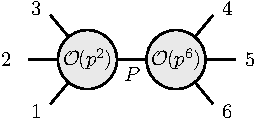
\includegraphics[trim={0cm 0cm 0cm 0cm},clip,scale=0.8]{p6-fac-3}} =A_4^{(2)}(123)\frac{1}{P^2}A_4^{(6)}(456)
$
\end{document}